\documentclass[problem]{mcs}

\begin{pcomments}
  \pcomment{MQ_coloring_short}
  \pcomment{excerpt from MQ_coloring}
\end{pcomments}

\pkeywords{
  coloring
  cycle
  chromatic_number
}

%%%%%%%%%%%%%%%%%%%%%%%%%%%%%%%%%%%%%%%%%%%%%%%%%%%%%%%%%%%%%%%%%%%%%
% Problem starts here
%%%%%%%%%%%%%%%%%%%%%%%%%%%%%%%%%%%%%%%%%%%%%%%%%%%%%%%%%%%%%%%%%%%%%

\begin{problem}
Determine a valid coloring of the graph shown in
Figure~\ref{fig:to_color} using as few colors as possible. (Simply
write your proposed color for each vertex next to that vertex.  You
may use $R$ for red, $G$ for green, etc.)

\begin{figure}[h]
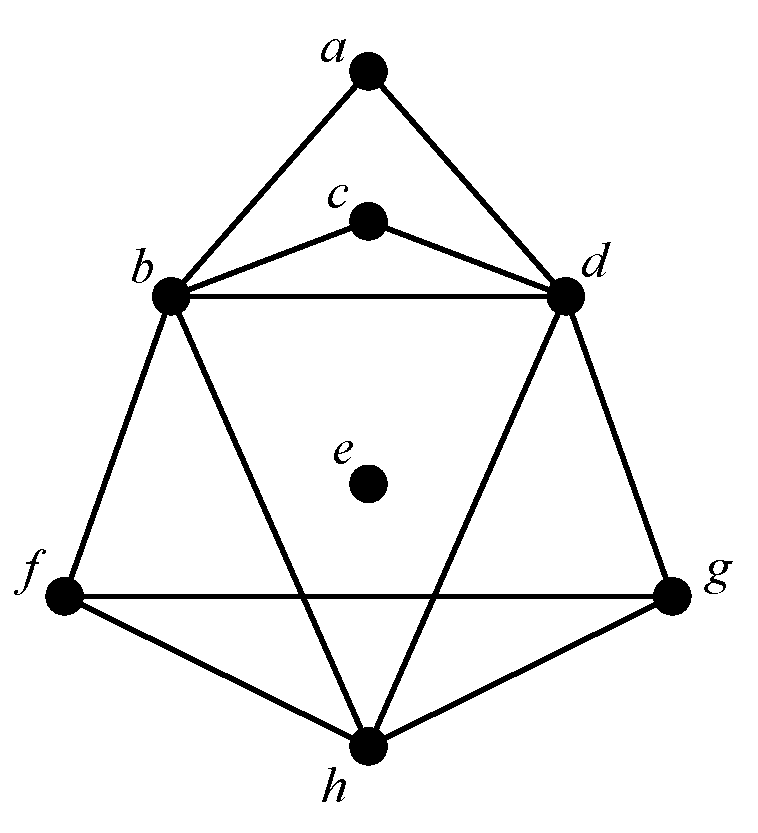
\includegraphics[width=0.4\linewidth]{MQ_coloring}
\caption{\label{fig:to_color}}
\end{figure}

\examspace[1in]

\begin{solution}
There are odd-length cycles in the graph, so at least three colors
will be needed.  So assume that three colors are sufficient.  (If we
encounter a contradiction under this assumption, we will need to use
more colors.)  Start with the length three cycle $abda$.  All of its
vertices must be colored differently, so assign red to $a$, blue to
$b$, and green to $d$.  The length three cycle $bdhb$ now forces $h$ to be
colored red.  $f$ must now be colored green and $g$ must be colored
blue.  The coloring is valid so far.  $c$ is adjacent to a blue vertex
and a green vertex, and no others, it must be colored red.  Finally,
$e$ is not adjacent to any other vertices, so it can be assigned any
of the three colors.  Choosing red for $e$, the result is shown in
Figure~\ref{fig:colored}.  There is no pair of like-colored adjacent
vertices, so this coloring is valid.

\begin{figure}[h]
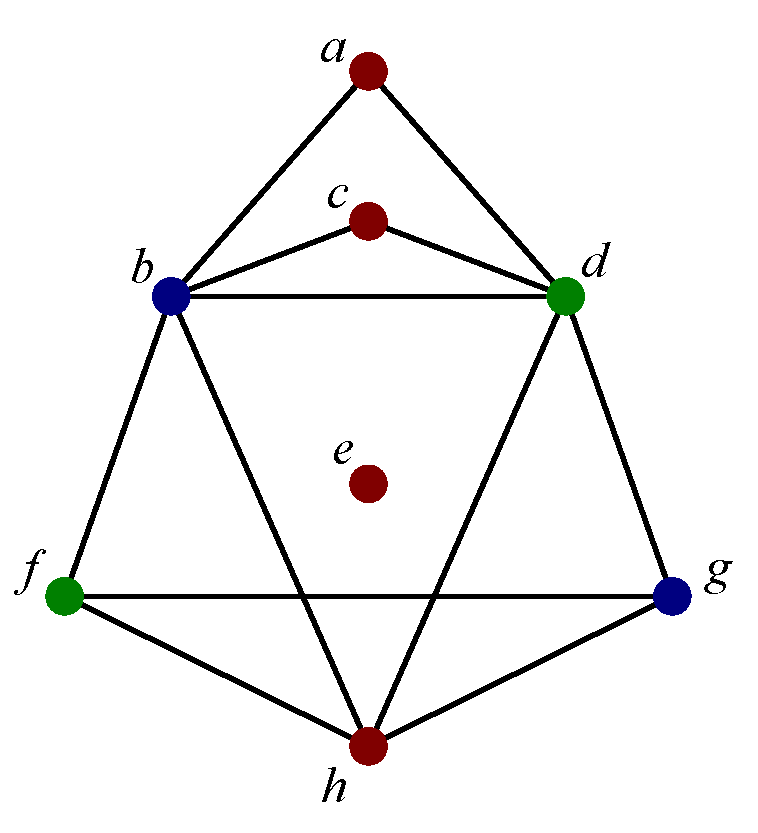
\includegraphics[width=0.4\linewidth]{MQ_coloring_sol}
\caption{A valid coloring.}
\label{fig:colored}
\end{figure}
\end{solution}

\end{problem}

\endinput
